
\subsubsection{Hermitian conjugate operator}

\begin{definition}
    Suppose $A$ is any linear operator on a Hilbert space, $V$. It turns out that there exists a unique linear operator $A^{\dagger}$ on $V$ such that for all vectors $|v\rangle,|w\rangle \in V$,
$$
(|v\rangle, A|w\rangle)=\left(A^{\dagger}|v\rangle,|w\rangle\right).
$$
This linear operator is known as the \textit{adjoint} or \textit{Hermitian conjugate} of the operator $A$. 
\end{definition}

From the definition it is easy to see that $(A B)^{\dagger}=B^{\dagger} A^{\dagger}$. 

By convention, if $|v\rangle$ is a vector, then we define 
$$
|v\rangle^{\dagger} \equiv\langle v|. 
$$
With this definition it is not difficult to see that $(A|v\rangle)^{\dagger}=\langle v| A^{\dagger}.$

\begin{remark}
    We verify the well-definedness of equation $(A|v\rangle)^{\dagger}=\langle v| A^{\dagger}$. Recall that we had defined the notation $\langle v|$ for the dual vector to the vector $|v\rangle$, which is a linear operator from $V$ to the complex numbers $\mathbf{C}$ by $\langle v|(|w\rangle) \equiv\langle v | w\rangle \equiv(|v\rangle,|w\rangle).$ Because $A^{\dagger} \colon V \to V$ and $\langle v | \colon V \to \mathbf{C}$, we have $\langle v| A^{\dagger}\colon V \to \mathbf{C}.$
\end{remark}

\begin{exercise}
Exercise 2.13: If $|w\rangle$ and $|v\rangle$ are any two vectors, show that $(|w\rangle\langle v|)^{\dagger}=|v\rangle\langle w|$.
\end{exercise}

\begin{exercise}
Exercise 2.14: (Anti-linearity of the adjoint) Show that the adjoint operation is \textit{anti-linear},
$$
\left(\sum_{i} a_{i} A_{i}\right)^{\dagger}=\sum_{i} a_{i}^{*} A_{i}^{\dagger}.
$$
\end{exercise}

\begin{exercise}
Exercise 2.15: Show that $\left(A^{\dagger}\right)^{\dagger}=A$.
\end{exercise}

In a matrix representation of an operator $A$, the action of the Hermitian conjugation operation is to take the matrix of $A$ to the conjugate-transpose matrix, $A^{\dagger} \equiv\left(A^{*}\right)^{T}$, where the $*$ indicates complex conjugation, and $T$ indicates the transpose operation. For example, we have
$$
\left[\begin{array}{cc}
1+3 i & 2 i \\
1+i & 1-4 i
\end{array}\right]^{\dagger}=\left[\begin{array}{cc}
1-3 i & 1-i \\
-2 i & 1+4 i
\end{array}\right]
$$

\subsubsection{Hermitian operator and projector}

An operator $A$ whose adjoint is $A$ is known as a \textit{Hermitian} or \textit{self-adjoint} operator. 

An important class of Hermitian operators is the \textit{projectors}. Suppose $W$ is a $k$-dimensional vector subspace of the $d$-dimensional vector space $V$. Using the Gram-Schmidt procedure it is possible to construct an orthonormal basis $|1\rangle, \ldots,|d\rangle$ for $V$ such that $|1\rangle, \ldots,|k\rangle$ is an orthonormal basis for $W$. By definition,
$$
P \equiv \sum_{i=1}^{k}|i\rangle\langle i|
$$
is the (orthogonal) projector onto the subspace $W$. It is easy to check that this definition is independent of the orthonormal basis $|1\rangle, \ldots,|k\rangle$ used for $W$. 

From the definition it can be shown that $|v\rangle\langle v|$ is Hermitian for any vector $|v\rangle$, so $P$ is Hermitian, $P^{\dagger}=P$. 

\begin{remark} %又是一种偷懒的写法
    We will often refer to the 'vector space' $P$, as shorthand for the vector space onto which $P$ is a projector. 
\end{remark}

The \textit{orthogonal complement of $P$} is the operator $Q \equiv I-P$. It is easy to see that $Q$ is a projector onto the vector space spanned by $|k+1\rangle, \ldots,|d\rangle$, which we also refer to as the orthogonal complement of $P$, and may denote by $Q$.

\begin{exercise}
    Exercise 2.16: Show that any projector $P$ satisfies the equation $P^{2}=P$.
\end{exercise}

\subsubsection{Normal operator }

An operator $A$ is said to be \textit{normal} if $A A^{\dagger}=A^{\dagger} A$. Clearly, an operator which is Hermitian is also normal. 

\textbf{There is a remarkable representation theorem for normal operators known as the spectral decomposition, which states that an operator is a normal operator if and only if it is diagonalizable.}

\begin{exercise}
Exercise 2.17: Show that a normal matrix is Hermitian if and only if it has real eigenvalues.
\end{exercise}

\subsubsection{Unitary operator}

A matrix $U$ is said to be \textit{unitary} if $U^{\dagger} U=I$. Similarly, an operator $U$ is unitary if $U^{\dagger} U=I$. It is easily checked that an operator is unitary if and only if each of its matrix representations is unitary (under arbitrary bases). 

\begin{remark}
    We can show that for a matrix $U$,  $U^{\dagger} U=I$ if and only if $U U^{\dagger} =I$. 
\end{remark}

A unitary operator also satisfies $U U^{\dagger}=I$, and therefore $U$ is normal and has a spectral decomposition. 

Geometrically, unitary operators are important because they \textbf{preserve inner products} between vectors. To see this, let $|v\rangle$ and $|w\rangle$ be any two vectors. Then the inner product of $U|v\rangle$ and $U|w\rangle$ is the same as the inner product of $|v\rangle$ and $|w\rangle$,
$$
(U|v\rangle, U|w\rangle)=\left\langle v\left|U^{\dagger} U\right| w\right\rangle=\langle v|I| w\rangle=\langle v | w\rangle.
$$

This result suggests the following elegant outer product representation of any unitary $U$. Let $\left|v_{i}\right\rangle$ be any orthonormal basis set. Define $\left|w_{i}\right\rangle \equiv U\left|v_{i}\right\rangle$, so $\left|w_{i}\right\rangle$ is also an orthonormal basis set, since unitary operators preserve inner products. Note that
$$
U=\sum_{i}\left|w_{i}\right\rangle\left\langle v_{i}\right|.
$$
Conversely, if $\left|v_{i}\right\rangle$ and $\left|w_{i}\right\rangle$ are any two orthonormal bases, then it is easily checked that the operator $U$ defined by $U \equiv \sum_{i}\left|w_{i}\right\rangle\left\langle v_{i}\right|$ is a unitary operator.

\begin{exercise}
    Exercise 2.18: Show that all eigenvalues of a unitary matrix have modulus 1, that is, can be written in the form $e^{i \theta}$ for some real $\theta$.
\end{exercise}

\begin{exercise}
    Exercise 2.19: (Pauli matrices: Hermitian and unitary) Show that the Pauli matrices are Hermitian and unitary.
\end{exercise}

\begin{exercise}
    Exercise 2.20: (Basis changes) Suppose $A^{\prime}$ and $A^{\prime \prime}$ are matrix representations of an operator $A$ on a vector space $V$ with respect to two different orthonormal bases, $\left|v_{i}\right\rangle$ and $\left|w_{i}\right\rangle$. Then the elements of $A^{\prime}$ and $A^{\prime \prime}$ are $A_{i j}^{\prime}=\left\langle v_{i}|A| v_{j}\right\rangle$ and $A_{i j}^{\prime \prime}=\left\langle w_{i}|A| w_{j}\right\rangle$. Characterize the relationship between $A^{\prime}$ and $A^{\prime \prime}$.
\end{exercise}

\subsubsection{Positive operator}

A special subclass of Hermitian operators is extremely important. This is the positive operators. 

A \textit{positive} operator $A$ is defined to be an operator such that for any vector $|v\rangle$, $(|v\rangle, A|v\rangle)$ is a real, non-negative number. If $(|v\rangle, A|v\rangle)$ is strictly greater than zero for all $|v\rangle \neq 0$ then we say that $A$ is \textit{positive definite}. 

Any positive operator is automatically Hermitian, and therefore by the spectral decomposition has diagonal representation $\sum_{i} \lambda_{i}|i\rangle\langle i|$, with non-negative eigenvalues $\lambda_{i}$.

\begin{remark}
    \textbf{Any positive operator is automatically Hermitian!} This conclusion is \textit{false} for linear algebra over the real number field. Consider a non-symmetric matrix $A=\left(\begin{array}{cc}
1 & 1 \\
-1 & 1
\end{array}\right)$ with the property that $v^{\top} A v \geq 0$ whenever $v \in \mathbf{R}^2.$ Again, there are quite a few conclusions that differ between linear algebra based on complex number field and those based on the real number field.
\end{remark}

\begin{exercise}
Exercise 2.21: Repeat the proof of the spectral decomposition in Box 2.2 for the case when $M$ is Hermitian, simplifying the proof wherever possible.
\end{exercise}

\begin{exercise}
Exercise 2.22: Prove that two eigenvectors of a Hermitian operator with different eigenvalues are necessarily orthogonal.
\end{exercise}

\begin{exercise}
Exercise 2.23: Show that the eigenvalues of a projector $P$ are all either 0 or 1.
\end{exercise}

\begin{exercise}
Exercise 2.24: (Hermiticity of positive operators) Show that a positive operator is necessarily Hermitian. (Hint: Show that an arbitrary operator $A$ can be written $A=B+i C$ where $B$ and $C$ are Hermitian.)
\end{exercise}

\begin{exercise}
Exercise 2.25: Show that for any operator $A, A^{\dagger} A$ is positive.
\end{exercise}

\subsubsection{Box 2.2: The spectral decomposition - important!}

The spectral decomposition is an extremely useful representation theorem for normal operators.

\begin{theorem}
    Theorem 2.1: (Spectral decomposition) Any normal operator $M$ on a vector space $V$ is diagonal with respect to some orthonormal basis for $V$. Conversely, any diagonalizable operator is normal.
\end{theorem}
%下面的证明只是参考,建议自行在网上查找其他类似的证明,可能更容易读。
\begin{proof}
    The converse is a simple exercise, so we prove merely the forward implication, by induction on the dimension $d$ of $V$. The case $d=1$ is trivial. Let $\lambda$ be an eigenvalue of $M, P$ the projector onto the $\lambda$ eigenspace, and $Q$ the projector onto the orthogonal complement. Then $M=(P+Q) M(P+Q)=P M P+Q M P+$ $P M Q+Q M Q$. Obviously $P M P=\lambda P$. Furthermore, $Q M P=0$, as $M$ takes the subspace $P$ into itself. We claim that $P M Q=0$ also. To see this, let $|v\rangle$ be an element of the subspace $P$. Then $M M^{\dagger}|v\rangle=M^{\dagger} M|v\rangle=\lambda M^{\dagger}|v\rangle$. Thus, $M^{\dagger}|v\rangle$ has eigenvalue $\lambda$ and therefore is an element of the subspace $P$. It follows that $Q M^{\dagger} P=0$. Taking the adjoint of this equation gives $P M Q=0$. Thus $M=P M P+Q M Q$. Next, we prove that $Q M Q$ is normal. To see this, note that $Q M=Q M(P+Q)=Q M Q$, and $Q M^{\dagger}=Q M^{\dagger}(P+Q)=Q M^{\dagger} Q$. Therefore, by the normality of $M$, and the observation that $Q^{2}=Q$,
$$
\begin{aligned}
Q M Q Q M^{\dagger} Q & =Q M Q M^{\dagger} Q \\
& =Q M M^{\dagger} Q \\
& =Q M^{\dagger} M Q \\
& =Q M^{\dagger} Q M Q \\
& =Q M^{\dagger} Q Q M Q
\end{aligned}
$$
so $Q M Q$ is normal. By induction, $Q M Q$ is diagonal with respect to some orthonormal basis for the subspace $Q$, and $P M P$ is already diagonal with respect to some orthonormal basis for $P$. It follows that $M=P M P+Q M Q$ is diagonal with respect to some orthonormal basis for the total vector space.
\end{proof}

In terms of the outer product representation, this means that $M$ can be written as $M=\sum_{i} \lambda_{i}|i\rangle\langle i|$, where $\lambda_{i}$ are the eigenvalues of $M,|i\rangle$ is an orthonormal basis for $V$, and each $|i\rangle$ an eigenvector of $M$ with eigenvalue $\lambda_{i}$. In terms of projectors, 
$$
M=\sum_{i} \lambda_{i} P_{i},
$$
where $\lambda_{i}$ are again the eigenvalues of $M$, and $P_{i}$ is the projector onto the $\lambda_{i}$ eigenspace of $M$. These projectors satisfy the completeness relation $\sum_{i} P_{i}=I$, and the orthonormality relation $P_{i} P_{j}=\delta_{i j} P_{i}$.

\subsubsection{Summary} %要仔细地品味和思考下面这些结论之间的关系
\begin{enumerate}
    \item all eigenvalues of a unitary operator have modulus 1
    \item a normal operator is Hermitian if and only if it has real eigenvalues.
    \item Pauli matrices are Hermitian and unitary.
    \item Any positive operator is automatically Hermitian
    \item all eigenvalues of a positive operator are non-negative
    \item the eigenvalues of a projector $P$ are all either 0 or 1.
\end{enumerate}

\begin{figure}[h]
    \centering
    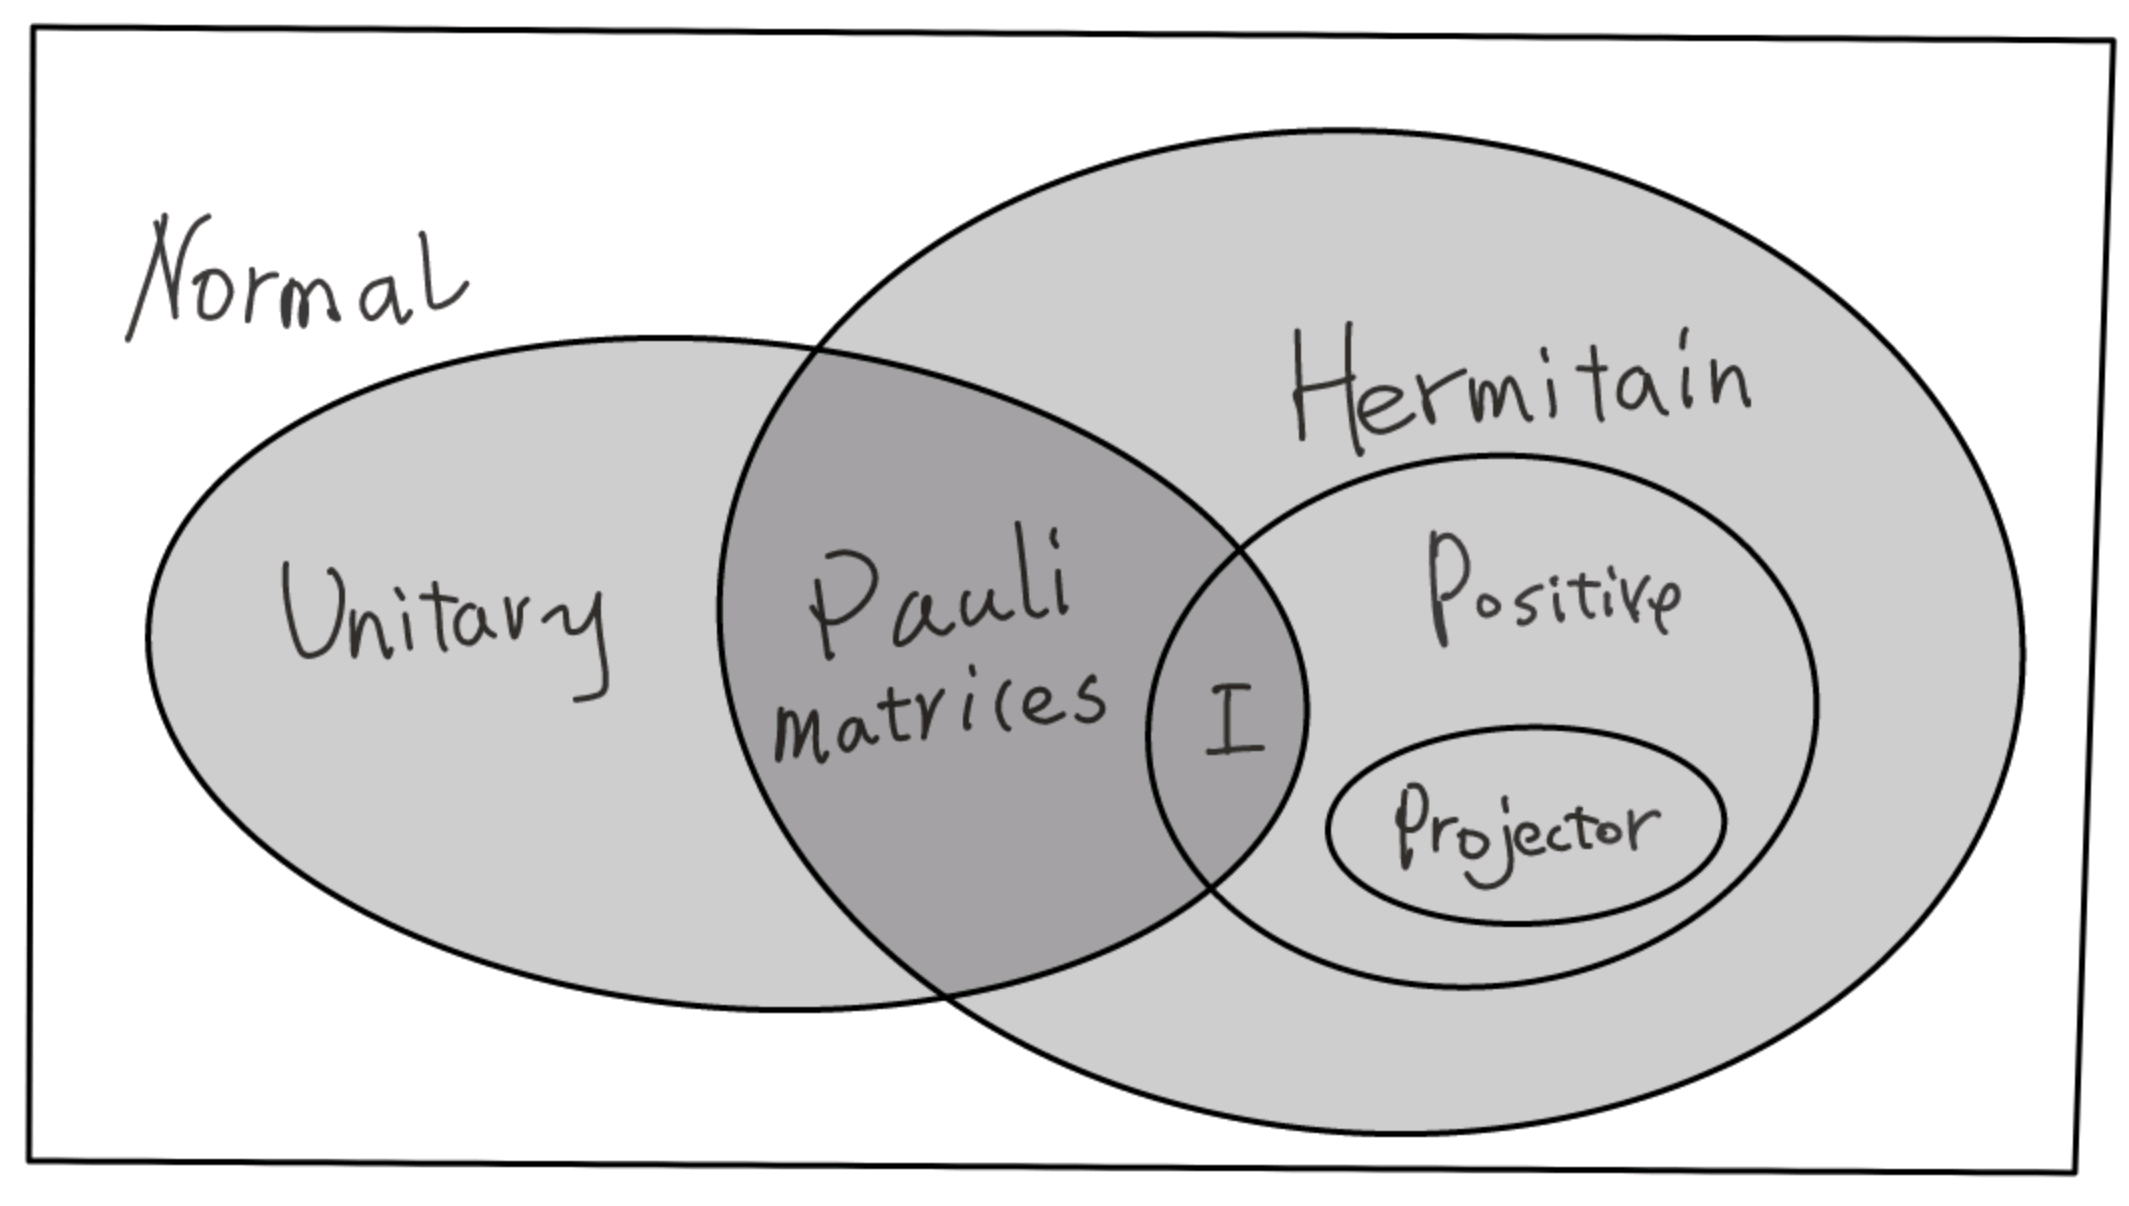
\includegraphics[width=0.75\linewidth]{Images/relations of many operators.png}
    \caption{\textbf{relations of many operators} }
\end{figure}